% !TeX root = /home/jakubp/Storage/OneDrive/Documents/Studies/masters/master_thesis/thesis.tex

\chapter{Krylov subspace methods for quantum many-body systems\label{chap:krylov}}
\thispagestyle{chapterBeginStyle}

One of the two purposes of this thesis is to develop and test a set of numerical tools based on the Krylov subspace methods,
which is a family of \textbf{iterative} methods concerned with projecting high dimensional problems into smaller dimension subspaces
and solving them therein. Given a finite dimensional vector space \(V \cong \CC^m \), a vector \(\vectorbold{v}\in \CC^m\) and
a linear operator \(A\in\CC^{m\cross m}\), represented as a matrix, the \textbf{k-th Krylov subspace} \(\K{k}\) is defined as 
\begin{equation}
		\K{k} := \mathrm{span}\{\,\vectorbold{v}, A\vectorbold{v}, A^2\vectorbold{v},\ldots,A^{k-1}\vectorbold{v} \,\} \subseteq \CC^m
	\label{def:krylov}
\end{equation}
Maximal dimension of a Krylov subspace is bounded from above by \(\mathrm{rank}(A) + 1\)~\autocite{Simoncini2015}.

This chapter serves as a
pedagogical introduction to the core ideas of these methods, including some of the usually omitted mathematical details.
For the initial part of this exposition we follow the excellent textbook of numerical linear algebra by~\textcite{Trefethen1997},
whereas for further applications to quantum many-body physics we rely on the excellent treatments of the topic
found in~\textcite{Sandvik2010} and PhD thesis by~\textcite{Crivelli2016}.

We start this chapter by quickly sketching the problems with \textbf{direct} algorithms such as Exact Diagonalization (ED), and quickly
follow with the fundamental iterative algorithm for sparse nonhermitian matrices, the Arnoldi iteration. Its output admits several
possible interpretations, however we shall focus on the problem of locating extremal eigenvalues.
Afterwards, we restrict our attention to the class of hermitian matrices, to which of course all typical tigh-binding Hamiltonians
belong to, and describe the Lanczos algorithm, which allows for efficient calculation of the ground state eigenvalue and eigenvector,
and thus the ground state properties of a system.
Yet in this work we are mainly interested in infinite temperature calculations, for which in principle sampling of the whole
spectrum is required. To this end, in subsequent sections we develop a scheme for time evolution of arbitrary state,
called the Krylov propagator~\autocite{Park1986}, and in the last section combine it with the idea of Dynamical Quantum Typicality (DQT),
which states that a single pure state can have the same properties as an ensemble density matrix~\autocite{Gemmer2003,Goldstein2006,Popescu2006}.
This will produce a numerical algorithm for efficient calculation of time dependent correlation functions without the need
for Exact Diagonalization.
% We finish this chapter with a proposal of employing this method to the identification of local integrals of motion in a given
% tight-binding system\autocite{Mierzejewski2015a}.
%  For the remainder of this chapter, let \(H\) denote arbitrary tight-binding Hamiltonian, \(\mathcal{H}\) the associated Hilbert space,
%  and \(\dimension = \textrm{dim}\left(\mathcal{H}\right) < \infty\) its dimension.

 \section{Problems with Exact Diagonalization}

 \begin{figure}[htbp]
	\centering
	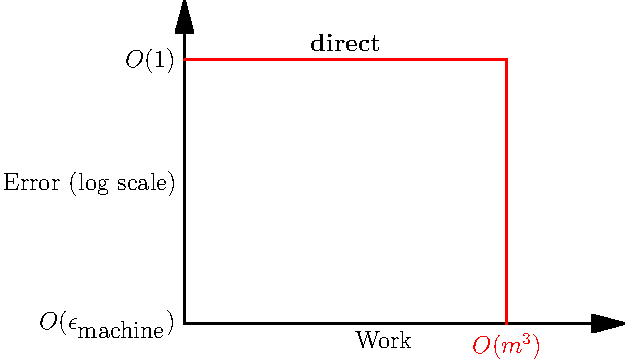
\includegraphics{Figures/direct_iterative.pdf}
	\caption{Schematic representatation of difference between direct (such as Exact Diagonalization) and
	iterative (such as Lanczos iteration) algorithms. The advantage of iterative methods comes from the fact that they
	can be stopped midway, after desired precision is reached. On the other hand, direct algorithms require all \(O(m^3)\)
	operations before any results can be extracted. Figure reproduced from~\textcite{Trefethen1997}.}
	\label{fig:direct_iter}
\end{figure}

  The most straightforward numerical method for studying discrete quantum many-body systems is without a doubt
 Exact Diagonalization (ED)~\autocite{Weisse2008}. It belongs to the family of the so-called direct algorithms (cf. Fig~\ref{fig:direct_iter})
and allows one to obtain numerically exact set of eigenvalues and eigenvectors and subsequently compute any desired properties
 of the system, be it thermal expectation values, time evolution, Green's functions etc. Unfortunately, the starting point of any
 ED calculation is the expression of the Hamiltonian as a dense matrix, in the Hilbert space basis of choice. Taking into account
 the fact that the dimension many-body Hilbert space grows exponentially with the size of the system, the memory cost quickly becomes
 prohibitive, even when exploiting conservation laws and related symmetries. For example, in the case of a spin chain of length L, with 
 on-site basis dimension being 2, the full dimension of the Hilbert space would be \(\dimension = 2^{L}\). Taking a modest length of 25 sites, that gives
 \(2^{25} = 33554432\approx 3.36 \cdot 10^7\) basis states and a memory footprint of Hamiltonian matrix of around 9PB (using double-precision
 floating point numbers), which is 9000 times more than the typical consumer hard drive capacity of 1TB. Even assuming some kind of distributed
 memory platform allowing for handling such large matrices, the computational complexity of ED, requiring \(O(\dimension^3)\) operations,
 is the next major hurdle. Therefore, it is exceedingly
 difficult to probe the thermodynamic limit physics and ED calculations suffer from finite size effects.
 
\begin{figure}[htbp]
	\centering
	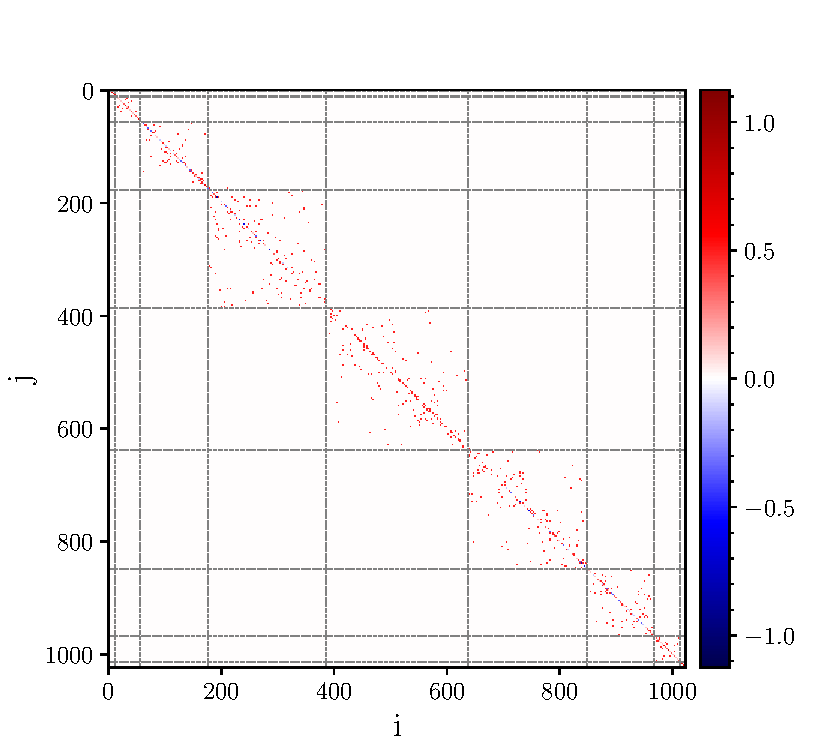
\includegraphics[width=0.7\linewidth]{Figures/matrix_elements.pdf}
	\caption{Ising basis representation of matrix of the XXZ Hamiltonian \(H = J\sum_{i} \left[\frac{1}{2}\left(\Sp_i \Sm_{i+1} +
	 \Sm_{i}\Sp_{i+1}\right) + \Delta \Sz_i \Sz_{i+1}\right]\) on \(10\) sites, with \(J = 1\) and \(\Delta=0.5\).
	Basis states are sorted according to the magnetization which yields the block structure emphasized by dashed lines.
	The filling factor \(\mu\) is approximately \(0.005\).}
	\label{fig:sparse_structure}
\end{figure}

 Closer investigation of the Hamiltonian matrix, expressed in computational basis\footnote{For spin systems, it is the eigenbasis of \(\Sz\) operator, also called the Ising basis.}
 quickly reveals the inefficiency of dense storage. Looking at Figure~\ref{fig:sparse_structure}, we see that most of
 the matrix elements are zero. In fact only about \(\mu \propto \dimension \) out of \(\dimension^2\) matrix elements
 are non-zero. Hence, a numerical scheme leveraging this sparsity is highly desirable. This is exactly what the Krylov subspace algorithms
 do, by the virtue of requiring only a "black box" computation of matrix-vector product, which can be fairly easily implemented in a way
 requiring only \(O(\mu \dimension)\) operations.

\section{Calculation of ground state}
Our goal in this section is to develop the Lanczos algorithm for ground state search of hermitian matrices, and along
the way understand how and why it works.

\subsection{Arnoldi iteration}
The Lanczos algorithm is special case of a more general algorithm, called Arnoldi iteration, designed to transform
a general, nonhermitian matrix \(A\in \CC^{m\cross m} \) via a orthogonal
\footnote{Orthogonal in this context means that \(Q^{\dagger}Q = I_{m \cross m}\)} similarity transformation to a Hessenberg form \(A = QHQ^{\dagger}\).
Such transformation always exist~\autocite{Garcia2017}. A square, \(m \cross m\) matrix \(H\) is said to be 
in \textbf{upper Hessenberg form} if \(\forall i,j\in \{\,1,\ldots,n\,\}: i > j+1 \implies (A)_{i,j}=0 \).
It is said to be in \textbf{lower Hessenberg form}, if its transpose is in upper Hessenberg form.
A Hessenberg matrix differs from a triangular one by one additional super- or subdiagonal.
Such form is desirable, because many numerical algorithms in linear algebra experience considerable speedup
from leveraging triangular structure of a matrix, and sometimes those benefits carry over to this almost-triangular
case. A particularly important strength of the Arnoldi iteration is that it can be interrupted before completion (cf. fig 32.1),
thus producing only an approximation of the Hessenberg form in situation where \(m\) is so large, that
full computations are infeasible (eg. in quantum many-body physics).

Assume now that we are able to only compute the first \(n < m\) columns of the equation \(AQ=QH\).
Let \(Q_n\) be the restriction of \(Q\) to \(n\) columns and let them be denoted by \(\vectorbold{q_1},\vectorbold{q_2}, \ldots 
\vectorbold{ q_n}\in \CC^m\).
Denoting by \(\tilde{H}_n\) the \((n+1)\cross n\) upper left section of H, which is also a Hessenberg matrix, we can 
write down the following \(n\)-step approximation to the full decomposition
\begin{equation}
	AQ_{n}=Q_{n+1}\tilde{H}_{n}
	\label{eq:krylov_n_approx}
\end{equation}
From this equation we can deduce an \(n+1\) term recurrence relation for the column \(\vectorbold{q_{n+1}}\), however
it is perhaps best illustrated with a simple example in the first place.

\begin{example}
	Let \(A\in \CC^{3\cross 3}\), \(AQ=QH\) be the Hessenberg decomposition and corresponding matrix elements
	be denoted by lowercase letters. We consider the approximation for \(n = 2\), i.e. \(AQ_2 = Q_3 \tilde{H}_2\).
	On the right hand side
	\begin{align*}
		AQ_2 = 
		\begin{bmatrix}
			a_{11} & a_{12} & a_{13} \\
			a_{21} & a_{22} & a_{23} \\
			a_{31} & a_{32} & a_{33}
			\end{bmatrix}
			\begin{bmatrix}
			q_{11} & q_{12} \\
			q_{21} & q_{22} \\
			q_{31} & q_{32}
			\end{bmatrix}
			&=
			\begin{bmatrix}
			a_{11}q_{11} + a_{12}q_{21} + a_{13}q_{31} & a_{11}q_{12} + a_{12}q_{22} + a_{13}q_{32} \\
			a_{21}q_{11} + a_{22}q_{21} + a_{23}q_{31} & a_{21}q_{12} + a_{22}q_{22} + a_{23}q_{32} \\
			a_{31}q_{11} + a_{32}q_{21} + a_{33}q_{31} & a_{31}q_{12} + a_{32}q_{22} + a_{33}q_{32}
			\end{bmatrix} \\
			&=
			\begin{bmatrix}
				(A\vectorbold{q_1})_1 & (A\vectorbold{q_2})_1 \\
				(A\vectorbold{q_1})_2 & (A\vectorbold{q_2})_2 \\
				(A\vectorbold{q_1})_3 & (A\vectorbold{q_2})_3
			\end{bmatrix}
	\end{align*}
	On the left hand side
	\begin{align*}
		Q_3 H_2 = 
		\begin{bmatrix}
			q_{11} & q_{12} & q_{13} \\
			q_{21} & q_{22} & q_{23} \\
			q_{31} & q_{32} & q_{33}
			\end{bmatrix}
			\begin{bmatrix}
			h_{11} & h_{12} \\
			h_{21} & h_{22} \\
			0 & h_{32}
			\end{bmatrix}
			&=
			\begin{bmatrix}
				q_{11}h_{11} + q_{12}h_{21} & q_{11}h_{12} + q_{12}h_{22} + q_{13}h_{32} \\
				q_{21}h_{11} + q_{22}h_{21} & q_{21}h_{12} + q_{22}h_{22} + q_{23}h_{32}\\
				q_{31}h_{11} + q_{32}h_{21} & q_{31}h_{12} + q_{32}h_{22}+ q_{33}h_{32}
			\end{bmatrix}\\		
			&=
			\begin{bmatrix}
				h_{11}(\vectorbold{q_1})_1 + h_{21}(\vectorbold{q_2})_1 & h_{12}(\vectorbold{q_1})_1 + h_{22}(\vectorbold{q_2})_1 + h_{32}(\vectorbold{q_3})_1 \\
				h_{11}(\vectorbold{q_1})_2 + h_{21}(\vectorbold{q_2})_2 & h_{12}(\vectorbold{q_1})_2 + h_{22}(\vectorbold{q_2})_2 + h_{32}(\vectorbold{q_3})_2 \\
				h_{11}(\vectorbold{q_1})_3 + h_{21}(\vectorbold{q_2})_3 & h_{12}(\vectorbold{q_1})_3 + h_{22}(\vectorbold{q_2})_3 + h_{32}(\vectorbold{q_3})_3
			\end{bmatrix}
	\end{align*}
	From the above calculation and~\ref{eq:krylov_n_approx} we can read off two identities
	\begin{align*}
		A\vectorbold{q_1} &= h_{11}\vectorbold{q_1}+h_{21}\vectorbold{q_2}\\
		A\vectorbold{q_2} &= h_{21}\vectorbold{q_1}+h_{22}\vectorbold{q_2} + h_{32}\vectorbold{q_3}
	\end{align*}
	Therefore we get, assuming \(\vectorbold{q_1}\) is known,
	\begin{align*}
		\vectorbold{q_2} &= \frac{A \vectorbold{q_1} - h_{11} \vectorbold{q_1}}{h_{21}}\\
		\vectorbold{q_3} &= \frac{A \vectorbold{q_2} - h_{21} \vectorbold{q_1} - h_{22}\vectorbold{q_2}}{h_{32}}
	\end{align*}
\end{example}
Generalizing the above example, we arrive at the desired \(n+1\) term recurrence relation for \(\vectorbold{q_{n+1}}\)
\begin{equation}
	\vectorbold{q_{n+1}} = \frac{A \vectorbold{q_n} - \sum_{m=1}^{n} h_{mn}\vectorbold{q_m}}{h_{n+1,n}}
	\label{eq:arnoldi_recurrence}
\end{equation}
We can now easily cast the above recurrence into a pseducode algorithm:
\begin{algorithm}
	\algrenewcommand\algorithmicrequire{\textbf{Input: }}
	\algrenewcommand\algorithmicensure{\textbf{Output: }}
	\caption{Arnoldi iteration}
	\label{alg:arnoldi}
	\begin{algorithmic}[1]
		\Require \(\vectorbold{v} \in \CC^m\), \(A \in \CC^{m\cross m}\), number of steps \(n\)
		\Ensure columns of \(Q_n\), matrix elements of \(H_n\)
		\State \(\vectorbold{q_1} = \vectorbold{v}/\norm*{\vectorbold{v}}\) \Comment{components of \(\vectorbold{v}\) are usually drawn from uniform distribution }
		\For{\(i = 1:n-1\)}
			\State \(\vectorbold{q} = A\vectorbold{q_i}\)
			\For{\(j = 1:i\)}
				\State \(h_{ji} = \mathrm{cdot}(\vectorbold{q_j},\vectorbold{q})\) \Comment{\(\mathrm{cdot}\) is the complex dot product on \(\CC^m\).}
				\State \(\vectorbold{q} = \vectorbold{q} - h_{ji}\vectorbold{q_j}\) \Comment{In exact arithmetic, this enusres orthogonality.}
			\EndFor
			\State \(h_{i+1,i} = \norm{\vectorbold{q}} \) 
			\State \(\vectorbold{q_{i+1}} = \vectorbold{q}/h_{i+1,i} \)
		\EndFor
	\end{algorithmic}
\end{algorithm}

Step 9 of the Algorithm~\ref{alg:arnoldi} may be questionable, as we are dividing by a norm of a vector, which
after all can be equal to zero. However, in practical applications of Arnoldi iteration it usually means
that our calculations have converged and the iterations may be stopped.


Examining closely the Arnoldi iteration algorithm, we notice that it is essentially the Gram-Schmidt
procedure applied to the vectors \(\{\,\vectorbold{v}, A\vectorbold{v},\ldots, A^{n-1}\vectorbold{v}\,\}\) and hence the 
vectors \(\{\,\vectorbold{q_1}, \vectorbold{q_2},\ldots,\vectorbold{q_n}\,\}\) form an orthonormal basis
of the Krylov subspace \(\K{n}\). The orthonormality condition is concisely expressed by 
the fact that \(Q^{\dagger}_n Q_{n+1} \) is the \(n\cross (n+1)\) identity matrix. Multiplying the left-hand side of
equation~\eqref{eq:krylov_n_approx} by \(Q^{\dagger}_n\) we get
\begin{equation}
	Q^{\dagger}_n A Q_n = \underbrace{Q^{\dagger}_n Q_{n+1}}_{\mathrm{Id}_{n\cross(n+1)}}\tilde{H}_n = H_n \in \CC^{n\cross n}
	\label{eq:hessenberg}
\end{equation}
where \(H_n\) is the Hessenberg matrix \(\tilde{H}_n\) with its last row removed. 

To understand the meaning
of matrix \(H_n\) from the point of view of linear algebra, consider the following reasoning. Imagine we are
given an endormophism of the space \(\CC^m\), represented in the standard basis by a matrix \(A\).
We would like to restrict it to a endormophism of the Krylov subspace \(\K{n},\; n < m\). Of course,
as \(\vectorbold{q} \in \K{n} \implies \vectorbold{q} \in \CC^m\), we can calculate the action of \(A\) on a vector
from Krylov subspace in a straightforward way. However, the resulting vector \(A\vectorbold{q}\) in not guaranteed
to be an element of \(\K{n}\). We need to orthogonally project it back to the subspace. Such projection
is realized by \(Q_n Q^{\dagger}_n \in \CC^{m\cross m}\) and hence, with respect to the standard basis on \(\CC^m\),
the desired restriction can be written as \(Q_n Q^{\dagger}_n A\). Transforming it to the basis given by columns of
\(Q_n\) we get \( Q_n^{-1}\left(Q_n Q^{\dagger}_n A\right)Q_n = Q^{\dagger}_n A Q_n\). Thus, matrix \(H_n\)
is the orthogonal projection of \(A\) to the subspace \(\K{n}\), represented in the basis
\(\{\,\vectorbold{q_1},\vectorbold{q_2},\ldots,\vectorbold{q_n}\,\}\).

\(H_n\) is once again a square matrix, so we can talk about its eigenvalues \(\{\theta_i\}_{i = 1}^n\)
in the usual fashion. These numbers are called the \textit{Arnoldi eigenvalues estimates at step \(n\)}, or
the \textit{Ritz values with respect to \(\K{n}\)}.
Given the interpretation above, we may suspect that they would be related to the eigenvalues of the original matrix \(A\).
Indeed, as we shall see in a moment, some of the Ritz values are extremally good approximations of some of the
original eigenvalues.


\subsection{Polynomial approximation and eigenvalues}

By carrying out the Arnoldi iterations for succesive steps, and at each step \(n\) (or at just some of the steps)
calculating the eigenvalues of the Hessenberg matrix \(H_n\), we are left with sequences of Ritz values. Some
of them often converge rapidly to, what we reasonably assume, eigenvalues of the original matrix \(A\).
However in practive, the maximal accessible \(n\) is much smaller than \(m\), so we cannot expect to find
all eigenvalues. As it turns out, Arnoldi iteration typically finds extremal eigenvalues, which fortunately
are those that we are interested in.

Before we will understand the details, let us introduce different, seemingly unrelated problem of 
\textit{polynomial approximation}. We can take any \(\vectorbold{q} \in \K{n}\) and using the 
defining basis of Krylov subspace \(\K{n}\)(Definition~\ref{def:krylov}), expand is as
\begin{align*}
	\vectorbold{q} &= a_0 \vectorbold{v} + a_1 A \vectorbold{v} + a_2 A^2 \vectorbold{v} + \ldots + a_{n-1} A^{n-1} \vectorbold{v} \nonumber \\
				   &= \left(a_0\Id + a_1 A + a_2 A^2 + \ldots + a_{n-1} A^{n-1}\right) \vectorbold{v}
\end{align*}
Utilizing the special structure of vectors from \(\K{n}\), we can define a polynomial \(p(z) = a_0
+ a_1 z + a_2 z^2 + \ldots + a_{n-1}z^{n-1}\), and concisely write our vector as \(\vectorbold{q} = p(A)\vectorbold{v}\).
As the vector \(\vectorbold{q}\) was arbitrary, we have estabilished an isomorphism between the \(n\)-th Krylov
subspace and the space of complex polynomials of maximal degree \(n-1\). We are now ready to state the problem:
\vspace{-0.3cm}
\begin{titled-frame}{Arnoldi Approximation Problem}
	\centering
Given a matrix \(A\in\CC^{m\cross m}\) and a vector \(\vectorbold{v}\in \CC^m\), find  
	\( p \in P^n := \{\, a_0 + a_1 z + \ldots + a_{n-1} z^{n-1} + z^n \mid a_0,a_1,\ldots a_{n-1}\in \CC \,\} \)\\
	such that \(\norm{p(A)\vectorbold{v}}_2\) is minimized.
\end{titled-frame}

Remarkably, the Arnoldi approximation is the exact solution to this problem. This fact is interesting enough that
we state it here as a theorem and, following~\textcite{Trefethen1997}, provide a complete proof.

\begin{theorem}
	If \(\textrm{dim}\left(\K{n}\right) = n\), i.e. matrix having columns \(\vectorbold{v},A\vectorbold{v},\ldots, A^{n-1}
	\vectorbold{v}\) is of rank \(n\), then the Arnoldi Approximation Problem has a unique solution \(p^n\in P^n\),
	given by the characteristic polynomial of the matrix \(H_n\), defined by~\eqref{eq:hessenberg}.
	\label{theorem:arnoldi_approximation}
\end{theorem}

\begin{proof}
	We start with an observation, that given a polynomial \(p\in P^n\), the vector \(p(A)\vectorbold{v}\)
	can be written as \(p(A)\vectorbold{v} = A^n \vectorbold{v} - Q_n \vectorbold{r}\) for some \(\vectorbold{r}\in \CC^n\).
	To see that, note that \(\left(A^n \vectorbold{v} - p(A)\vectorbold{v}\right) \in \K{n}\) and columns of \(Q_n\) form an
	orthonormal basis of \(\K{n}\). Now, we can recast our problem into a slighlty different language, namely finding a vector
	in \(\K{n}\) that is the closest in the sense of \(L_2\) norm to \(A^n \vectorbold{v}\). In short:
	\begin{equation*}
		\vectorbold{r}^{\ast} = \min_{\vectorbold{r}\in\CC^n}\norm*{A^n \vectorbold{v} - Q_n \vectorbold{r}}
	\end{equation*}
	To achieve that, we need to have \(p(A)\vectorbold{v}\perp \K{n}\), that is \(p(A)\vectorbold{v}\) must
	be orthogonal to all basis vectors spanning \(\K{n}\). This is consisely expressed as 
	\(Q^{\dagger}_{n} p(A)\vectorbold{v} = \vectorbold{0}\in \CC^n\).

	Now, we know that the Hessenberg factorization \(A = QHQ^{\dagger}\) exists, and is approximated by \(n\) steps
	of the Arnoldi iteration. Thus, the matrices \(Q\) and \(H\) can have the following block structure:
	\begin{equation}
		Q=\left[\begin{array}{ll}
			Q_n & V
			\end{array}\right],
			\quad H=\left[\begin{array}{cc}
			H_n & 0_{n\cross(m-n)} \\
			Y & 0_{(m-n)\cross(m-n)}
			\end{array}\right]
			\label{eq:block_matrices}
	\end{equation}
	where \(V \in \CC^{m\cross(m-n)}\) is a matrix with orthonormal columns, which are also orthogonal to columns of
	\(Q_n\), and matrix \(Y\in\CC^{(m-n)\cross n}\) has only the upper-right entry different from zero
	(the one from the last row of \(\tilde{H}_n\)). Using the Hessenberg factorization we can write our condition
	as \(Q_n^{\dagger} Q p(H) Q^{\dagger}\vectorbold{v} = \vectorbold{0}\), and because equation~\eqref{eq:block_matrices}
	introduces partitions into \textit{conformable} blocks, we can use the rules of block-matrix algebra to simiplify
	it further~\autocite{Eves1980}.

	First, let us investigare closely the structure of \(p(H)\). We observe that
	\begin{align*}
		H^2 &= \left[\begin{array}{cc}
			H_n & 0_{n\cross(m-n)} \\
			Y & 0_{(m-n)\cross(m-n)}
			\end{array}\right]^2 = 
			\left[\begin{array}{cc}
				H_n^2 & 0_{n\cross(m-n)} \\
				Y H_n & 0_{(m-n)\cross(m-n)}
			\end{array}\right]\\
		H^3 &=
			\left[\begin{array}{cc}
				H_n & 0_{n\cross(m-n)} \\
				Y & 0_{(m-n)\cross(m-n)}
			\end{array}\right]^3 = 
			\left[\begin{array}{cc}
				H_n^3 & 0_{n\cross(m-n)} \\
				Y H_n^2 & 0_{(m-n)\cross(m-n)}
			\end{array}\right]\\
			\ldots\\
		H^n &= 			\left[\begin{array}{cc}
			H_n & 0_{n\cross(m-n)} \\
			Y & 0_{(m-n)\cross(m-n)}
		\end{array}\right]^n = 
		\left[\begin{array}{cc}
			H_n^n & 	  0_{n\cross(m-n)} \\
			Y H_n^{n-1} & 0_{(m-n)\cross(m-n)}
		\end{array}\right]\\
	\end{align*}
Thus \(p(H)\) can be written as
\begin{align*}
	p(H) &= a_0 \Id + a_1 H + a_2 H^2 + \ldots + a_{n-1} H^{n-1} + H^n \\
		&= \left[\begin{array}{cc}
			a_0 \Id + a_1 H_n + a_2 H_n^2 + \ldots + a_{n-1} H_n^{n-1} + H_n^n & 0_{n\cross(m-n)}\\
			a_0 \Id + a_1 Y + a_2 Y H_n + \ldots + a_{n-1} Y H_n^{n-2} + Y H_n^{n-1} & 0_{(m-n)\cross(m-n)}
		\end{array}\right]\\
		&= \left[\begin{array}{cc}
			p(H_n) & 0\\
			\tilde{Y} & 0
		\end{array}\right]
\end{align*}
We have now all the pieces to simplify the orthogonality condition:
\begin{align*}
	\vectorbold{0} &= Q_n^{\dagger} Q p(H) Q^{\dagger}\vectorbold{v}\\
	&= \left[Q_n^{\dagger}\right] 
	\left[\begin{array}{cc}
		Q_n & V
	\end{array}\right]
	\left[\begin{array}{cc}
		p(H_n) & 0_{n\cross(m-n)}\\
		\tilde{Y} & 0_{(m-n)\cross(m-n)}
	\end{array}\right]
	\left[\begin{array}{cc}
		Q_n^{\dagger}\\
		U^{\dagger}
	\end{array}\right] \vectorbold{v}\\
	&= \left[\begin{array}{cc}
		\Id_{n\cross n} & 0_{n\cross(m-n)}
	\end{array}\right] 
	\left[\begin{array}{cc}
		p(H_n) & 0_{n\cross(m-n)}\\
		\tilde{Y} & 0_{(m-n)\cross(m-n)}
	\end{array}\right]
	\left[\begin{array}{cc}
		Q_n^{\dagger}\\
		U^{\dagger}
	\end{array}\right] \vectorbold{v}\\
	&= \left[\begin{array}{cc}
		p(H_n) & 0_{n\cross (m-n)} 
	\end{array}\right]
	\left[\begin{array}{cc}
		Q_n^{\dagger}\\
		U^{\dagger}
	\end{array}\right] \vectorbold{v}\\
	&= p(H_n)Q_n^{\dagger} \vectorbold{v}
\end{align*}
As a final step, notice that by construction the first row of \(Q_n^{\dagger}\) is
\(\vectorbold{v}/\norm{\vectorbold{v}}\), and all the remaining rows are orthogonal to \(\vectorbold{v}\),
therefore only the first column of \(H_n\), or the first \(n\) elements of the first column of \(H\) are required
to be \(0\). By Caylel-Hamilton theorem, this is guaranteed if we take \(p = p^n\), where \(p^n\) is the characteristic
polynomial of \(H_n\). For the uniqueness part, suppose that there exists another polynomial, say \(q^n\) such
that \(q^n \perp \K{n}\). But then \(p^n - q^n\) is a nonzero polynomial of degree \(n-1\) (because \(p^n,\;q^n\) are
monic) such that \((p^n-q^n)(A)\vectorbold{v}=\vectorbold{0}\), and hence vectors \(\vectorbold{v},A\vectorbold{v},\ldots, A^{n-1}
\vectorbold{v}\) are linearly dependent, which violates assumption that \(\textrm{dim}\left(\K{n}\right) = n\).
\end{proof}
This theorem allows us to interpret the Arnoldi eigenvalues estimates \(\{\theta_i\}\) as the roots of the optimal
polynomial. Following the above proof, it is relatively easy to see that they are scale invariant, i.e.
if \(A\to\alpha A\) for some \(\alpha\in\CC\), then \(\{\theta_i\}_{i=1}^n \to \{\alpha\theta_i\}_{i=1}^n\)
and invariant under unitary transformations, i.e. if \(A\to UAU^{\dagger}\) and \(\vectorbold{v}\to U\vectorbold{v}\) for
some unitary \(U\), then the Arnoldi estimates are unchanged. Furthermore, owing to the properties of monic polynomials,
they are also translationally invariant, namely if \(A\to A + \alpha \Id\) for some \(\alpha\in\CC\), then
\(\{\theta_i\}_{i=1}^n \to \{\theta_i + \alpha\}_{i=1}^n\).

In the end we see that the direct purpose of Arnoldi iteration is to solve a polynomial approximation problem
and not to find eigenvalues. However, those two problems have enough in common, that the Arnoldi iteration
produces some correct eigenvalues as a `by-product'. We can reason along the following lines. If our task
is to find a polynomial \(p\in P^n\) minimizing \(\norm{p(A)}\), it may be a good idea to select a polynomial
that has roots close to the eigenvalues of \(A\).  In an extreme situation, when there exists a diagonalization
of \(A\) and it posses only \(n\ll m\) distinct eigenvalues, the minimal polynomial\footnote{A minimal polynomial
of matrix \(A\) is a polynomial \(p\) of the smallest degree such that \(p(A) = 0\). It always divides the
characteristic polynomial.} will coincide with the characteristic polynomial computed via Arnoldi iteration
after \(n\) steps and the Arnoldi eigenvalue approximations will be exact,
provided we start from \(\vectorbold{v}\) having nonzero overlap with all eigenvectors of \(A\).
In most practical situations however, the agreement is only approximate, namely Arnoldi eigenvalues are close to real
eigenvalues, and computed polynomial is such that \(\norm{p(A)}\) is small.

There is more to this story than we have told here, particularly a nice geometric interpreation
of Algorithm~\ref{alg:arnoldi} via \textit{Arnoldi lemniscates}, which illustrates why extremal eigenvalues
are found first, however we shall not concern ourselves with those
matters any further. Interested readers are once again referred to~\textcite{Trefethen1997},
whereas we turn our attention to the case of utmost interest in quantum mechanics, namely Arnoldi iteration
for hermitian matrices.

\subsection{Restriction to hermitian matrices: Lanczos iteration}

After the mathematical detour of previous section, armed with deeper understanding of Krylov subspace and
Arnoldi iteration, we are now going to investigate the algorithms that are of direct relevance to condensed
matter physics, starting with Lanczos iteration. From this point onwards, we shall switch to the favored by physicsts
Dirac bra-ket notation, namely \(\ket{v} \equiv \vectorbold{v}\) and \(\bra{v} = \vectorbold{v}^{\dagger}\).
Moreover, we assume the matrix \(A\) to be hermitian,
as in most use cases it will be the Hamiltonian of our system. 

It immediately follows from~\eqref{eq:hessenberg} that, given \(A\) is hermitian, the Hessenberg matrix 
\(H_n\) will also be hermitian. But a matrix that is both Hessenberg and hermitian, must of course be tridiagonal!
Indeed, to see this directly, let us write the equation for matrix elements \((H_n)_{ij}\) of \(H_n\):
\begin{equation}
	(H_n)_{ij} = \sum_{r,s}(Q_n^{\dagger})_{ir}(A)_{rs}(Q_n)_{sj} = \matrixel{q_i}{A}{q_j}
	\label{eq:hess_mat_el}
\end{equation}
where \(\ket{q_i},\ket{q_j}\) are respectively \(i\)-th and \(j\)-th columns of matrix \(Q_n\). From 
the recurrence relation~\eqref{eq:arnoldi_recurrence} we know that 
\(A\ket{q_j} \in \mathrm{span}\{\ket{q_1},\ldots,\ket{q_{j+1}}\}\), and that it is orthogonal to all
\(\ket{q_i}\) with \(i > j+1\). Therefore \((H_n)_{ij} = 0\) for \(i>j+1\). Simiarly, by taking the hermitian conjugate
of equation~\eqref{eq:hess_mat_el}, we get
\begin{equation}
	(H_n)_{ij} = \matrixel{q_j}{A^{\dagger}}{q_i} \triangleq  \matrixel{q_j}{A}{q_i}	
\end{equation}
where \(\triangleq\) follows from assumed hermiticity of \(A\). Repeating the above reasoning we
quickly obtain that \((H_n)_{ij} = 0\) also for \(j > i+1\) and hence the matrix is tridiagonal.
In literature the diagonal is usually denoted by \(\alpha_i \equiv (H_n)_{ii}\), whereas the sub- and superdiagonal
are denoted by \(\beta_i \equiv (H_n)_{i,i+1} = (H_n)_{i+1,i}\). The relation for \(\ket{q_{n+1}}\) becomes
a \(3\)-step recurrence:
\begin{equation}
	\ket{q_{n+1}} = \frac{A \ket{q_n} - \beta_{n-1}\ket{q_{n-1}} - \alpha_n \ket{q_n}}{\beta_n}
	\label{eq:lanczos_recurrence}
\end{equation}
This has a tremendous impact on the practical applications of the algorithm, as both
computational and memory costs decrease significantly. We are now ready to state the simplified version of
the Algorithm~\ref{alg:arnoldi}.
\begin{algorithm}
	\algrenewcommand\algorithmicrequire{\textbf{Input: }}
	\algrenewcommand\algorithmicensure{\textbf{Output: }}
	\caption{Lanczos iteration}
	\label{alg:lanczos}
	\begin{algorithmic}[1]
		\Require  \(\ket{v} \in \CC^m\), \(A \in \CC^{m\cross m}\) such that \(A^{\dagger} = A\), number of steps \(n\)
		\Ensure columns of \(Q_n\), tridiagonal matrix \(H_n\)
		\State \(\beta_0 = 0\)
		\State \(\ket{q_0} = \vectorbold{0} \in \CC^m\)
		\State \(\ket{q_1} = \ket{v}/\norm*{\ket{v}}\)
		\For{\(i = 1:n-1\)}
			\State \(\ket{q} = A\ket{q_i}\)
			\State \(\alpha_i = \braket{q_i}{q}\)
			\State \(\ket{q} = \ket{q} - \beta_{i-1}\ket{q_{i-1}} - \alpha_i \ket{q_i}\)
			\State \(\beta_i = \norm{\ket{q}} \) 
			\State \(\ket{q_{i+1}} = \ket{q}/\beta_i \)
		\EndFor
	\end{algorithmic}
\end{algorithm}
Another important observation is that \(\alpha_n\)'s are diagonal elements of a hermitian matrix, and \(\beta_n\)'s are
norms of vector \(\ket{q}\) in subsequent interations, both of which are real. Therefore, even if our Hamiltonian is
complex, the numbers \(\alpha_n\) and \(\beta_n\) can be stored as vectors of real floating point numbers, decreasing
memory requirements even further. This is the first algorithm implemented for the purpose of this thesis, using
the Armadillo linear algebra library~\autocite{Sanderson2016} and Intel MKL.

Matrix \(Q_n\) is of dimension \(m \cross n\), so keeping it in full in the memory can still be costly. Fortunately,
at each step of the Lanczos iteration no more than three vectors are necessary (\(\ket{q},\ket{q_i},\ket{q_{i-1}}\))
so the storage of full matrix \(Q_n\) is reduntant. Extremal eigenvalues are then obtained by explicit diagonalization
of the constructed matrix \(H_n = V_n D_n (V_n)^{\dagger}\), which can be done efficiently using specialized routines
for tridiagonal matrices. However, this approach has it drawbacks when we are interested also in the ground state
eigenvector, which will be the case in further applications. 

It turns out that the Lanczos iteration can approximate not only eigenvalues,
but also corresponding eigenvectors. They are the eigenvectors of the tridiagonal matrix \(H_n\), transformed back
to the original Hilbert space. Given the full Hessenberg decomposition we would have
\begin{equation}
	A = Q H Q^{\dagger} = Q (VDV^{\dagger}) Q^{\dagger} = (QV)D(QV)^{\dagger}
	\label{eq:factorization}
\end{equation}
Restriction to \(n\)-step iteration produces an approximation \(A\approx (Q_n V_n)D_n(Q_n V_n)^{\dagger}\).
The simplest form of Lanczos iteration presented in Algorithm~\ref{alg:lanczos} is sufficient to obtain
only the ground state eigenvector with machine precision, because eigenvectors of excited states are plagued
by loss of orthogonality stemming from the nature of floating point numbers. We shall have a brief look at this problem
at the end of this section.

The ground state vector \(\ket{\psi_0}\) can be then read of as the first column \(Q_n V_n\). However, there is a problem.
To conserve memory, we have not constructred the whole matrix \(Q_n\) explicitly, but only three of its columns 
at a given time and hence do not have access to the matrix product \(Q_n V_n\). We need a second pass of the Lanczos
iteration, with a single line added for iteretive calculation of the first column. It can be summarized by the
following piece of pseducode:

\begin{algorithm}
	\algrenewcommand\algorithmicrequire{\textbf{Input: }}
	\algrenewcommand\algorithmicensure{\textbf{Output: }}
	\caption{Second pass of Lanczos iteration, for calculating ground state eigenvector}
	\label{alg:lanczos_second_pass}
	\begin{algorithmic}[1]
	\Require \(\ket{\psi_0} = \vectorbold{0} \in \CC^m\), matrix \(V_n\) from Alg.~\ref{alg:lanczos}, rest of input data from Alg.~\ref{alg:lanczos}
		\Ensure columns of \(Q_n\), tridiagonal matrix \(H_n\)
		\State \(\beta_0 = 0\)
		\State \(\ket{q_0} = \vectorbold{0} \in \CC^m\)
		\State \(\ket{q_1} = \ket{v}/\norm*{\ket{v}}\)
		\For{\(i = 1:n-1\)}
			\State \(\ket{\psi_0} = \ket{\psi_0} + (V_n)_{i,1}\ket{q_i}\) \Comment{this is the only difference from Alg.~\ref{alg:lanczos}}
			\State \(\ket{q} = A\ket{q_i}\)
			\State \(\alpha_i = \braket{q_i}{q}\)
			\State \(\ket{q} = \ket{q} - \beta_{i-1}\ket{q_{i-1}} - \alpha_i \ket{q_i}\)
			\State \(\beta_i = \norm{\ket{q}} \) 
			\State \(\ket{q_{i+1}} = \ket{q}/\beta_i \)
		\EndFor
	\end{algorithmic}
\end{algorithm}

To finish this section, let us discuss quickly the convergence properties of Lanczos iteration. We have one free parameter,
namely the number of iterations \(n\). If we had carried out the full Arnoldi iteration, as described in~\ref{alg:arnoldi},
the orthogonality of subsequent columns of matrix \(Q_n\) would be guaranteed by the explicit Gram-Schmidt procedure
and we in principle could continue it up to \(n = m\) obtaining the full Hessenberg decomposition. However, 
restricting ourselves to a three step recurrence in Lanczos iteration we rely on mathematical identities to
force the orthogonality of \(\ket{q_i}\) with all previous vectors. Those are valid in exact arithmetic, but can
quickly break down when using floating point numebers, as it is done in practice. Therefore, the iteration is unstable and
should be stopped as soon as desired accuracy is reached. Taking \(E_n^1\) to be the lowest eigenvalues of
\(H_n\), the convergence criterion can be defined as \(\abs{E_{n+1}^1 - E_{n}^1}/\abs{E_n^1} < \varepsilon\) for some
small \(\varepsilon\), e.g. \(10^{-14}\). As long as it is nondegenerate, the convergence usually happens quite quickly for
both lowest eigenvalue and corresponding eigenvector. To reliably obtain higher eigenstates one needs to perform
reorthogonalization, but it requires keeping the matrix \(Q_n\) in memory which can be very costly.

\begin{figure}[htbp]
	\centering
	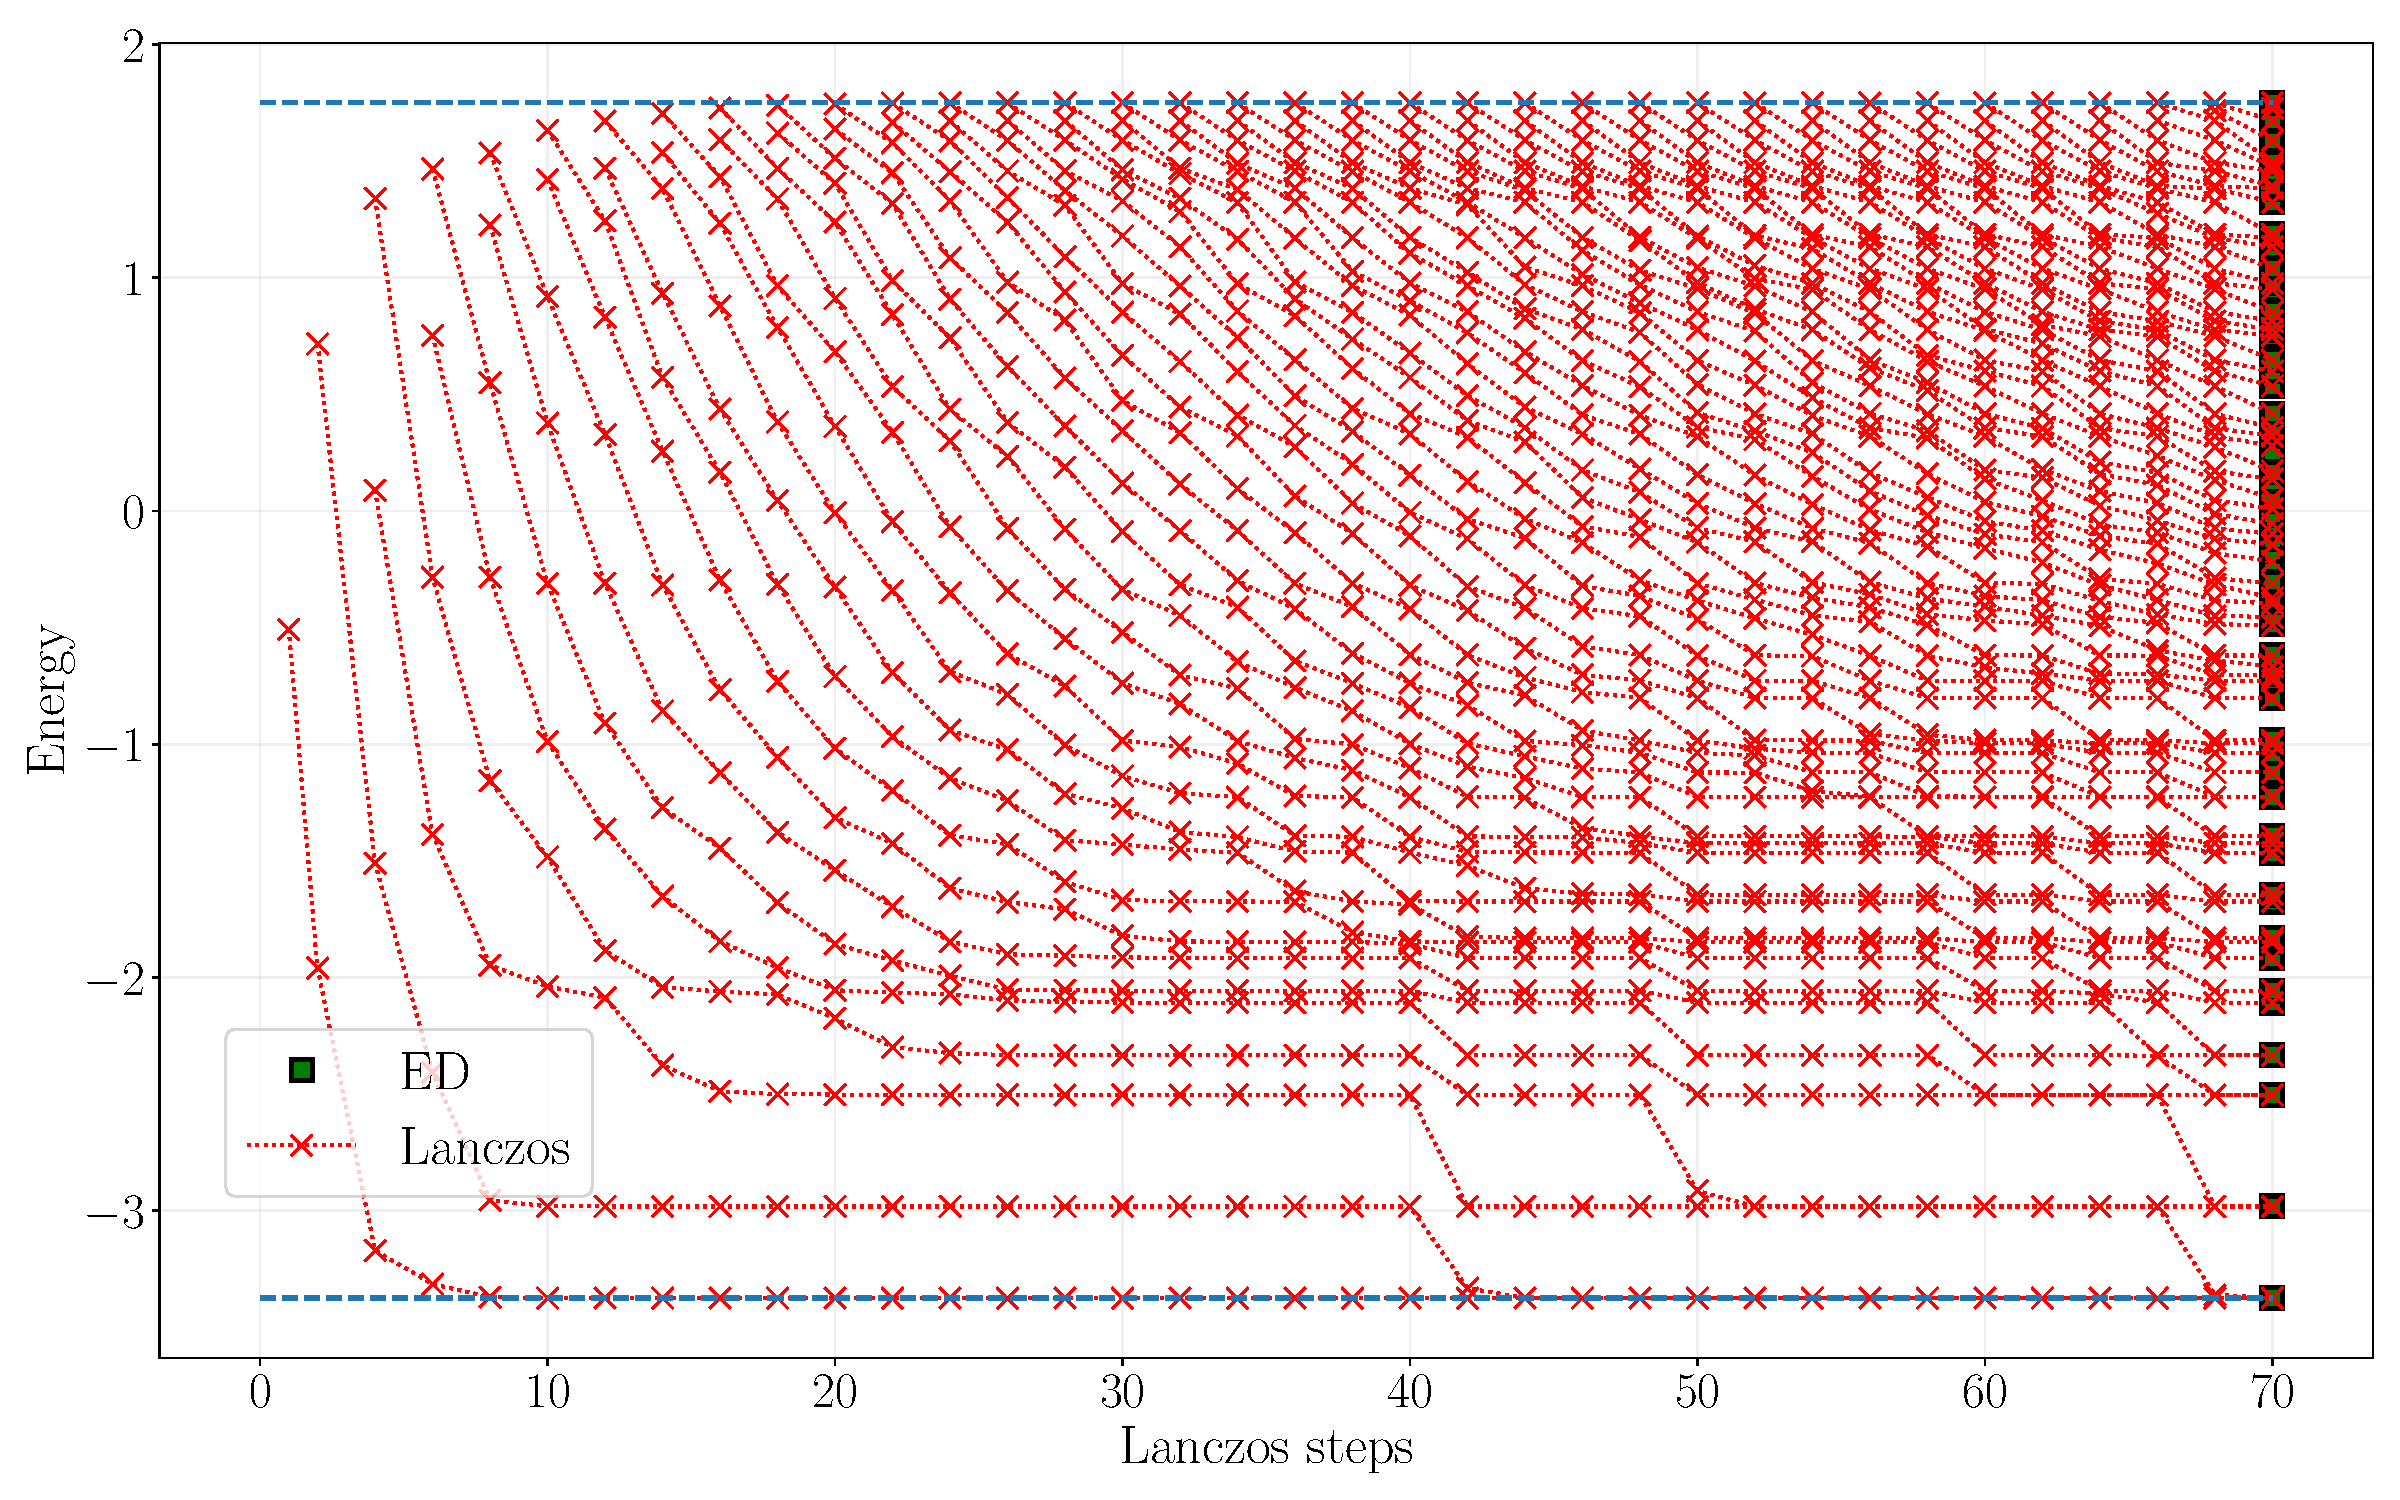
\includegraphics[width=\linewidth]{Figures/lanczos_L_8.pdf}
	\caption{Plot of Arnoldi eigenvalues as a function of Lanczos steps, for a XXZ chain on \(8\) sites in the
	subspace with \(0\) total magnetization. The extremal eigenvalues converge very quickly to the values matching
	Exact Diagonalization. The numerical instability of Lanczos iteration is especially visible for a few lowest
	eigenvalues, where mutliple ghosts start appearing. After \(\binom{8}{4} = 70\) Lanczos steps, 
	we should observe the exact spectrum emerging from Arnoldi approximates. However,
	we see that the ground state is triple degenerated, instead of unique as it should be.}
	\label{fig:ghosts}
\end{figure}

This instability can manifest itself in an interesting way, namely in form of additional eigenvalues, called Lanczos `ghosts'.
They are spurious copies of already found eigenvalues, which start apperating after too many iteration steps (cf. Fig.~\ref{fig:ghosts})
They are difficult to understand rigorously, however~\textcite{Trefethen1997} offer a nice heuristic explanatation.
Reaching convergence of some Arnoldi approximated eigenvalue to the true eigenvalue of A causes annihilation
of corresponding eigenvector component in the vector \(\ket{q}\). However, rounding errors originating from
floating point arithmetic cause \(\ket{q}\) to again develop component in the direction of the eigenvector
and thus, after certain number of iterations, appearance of another Arnoldi approximated eigenvalue is necessary
to annihilate it. This can go on and on producing more and more Lanczos 'ghosts'.
Fortunately, for all further applications in this thesis we will only require the lowest eigenstate, so we can
avoid most of the instability problems by stopping the iteration sufficiently quick.

\section{Time evolution via the Krylov propagator}

Even though the original puprose of Lanczos iteration was to approximate boundaries of the spectrum of matrices and
solve systems of linear equation~\autocite{Simoncini2016,Shewchuk1994a}, it can also be employed to evaluate functions
of hermitian matrices. Given any unitary (or orthogonal) decomposition of matrix \(A = QHQ^{\dagger}\), and an analytic
function \(f\)\footnote{A function \(f\) is real (complex) analytic if and only if its Taylor series about \(x_0\) 
converges in some neighborhood of \(x_0\) pointwise to the function, for every \(x_0\) in the domain.}, we have
\(f(A) = Qf(H)Q^{\dagger}\). And indeed, Lanczos iteration gives us such decomposition, albeit an approximate one
\(A \approx Q_n H_n Q_n^{\dagger}\). Because of this approximate character and convergence probles discussed at
the end of previous section, global approximation of \(f(A)\) via Lanczos iteration is a hopeless endevour.
However, the goal of this section is to calculate time evolution, which boils down to evaluation how the time-evolution
operator \(\exp\left(-i \hat{H} t\right) \) acts on some state \(\ket{v}\) in the Hilbert space for a given
Hamiltonian \(\hat{H}\). It is thus enough to restrict our attention the problem of calculating \(f(A){\ket{v}}\), for
which the Lanczos iteration turns out to be an excellent tool.

Let us now assume that the matrix \(A\) is our Hamiltonian \(\hat{H}\), acting on Hilbert space \(\mathcal{H}\cong \CC^m\)
and \(\ket{v}\in \mathcal{H}\) is some fixed state.
Using the approximate factorization derived from~\eqref{eq:factorization}, we get
\begin{equation}
	f(\hat{H})\ket{v} \approx (Q_n V_n) f(D_n) (Q_n V_n)^{\dagger} \ket{v} 
	\label{eq:fun_eval}
\end{equation}
where \(D_n\) is a real diagonal matrix, so \(f(D_n)\) is easy to compute.
Previously, we have started the construction of Krylov subspace basis from some random vector. Now, let us
change this slighlty and start from the vector \(\ket{v}\) instead, which we assume to be normalized. Then,
the first column of \(Q_n\) will be \(\ket{v}\), whereas all subsequent columns will be orthogonal (up to some
numerical errors), yielding \(Q_n^{\dagger}\ket{v} = \ket{e_1}\), which is the first vector in canonical basis
of \( \CC^n \), i.e. \( \ket{e_1} = \left[1,0,0,\ldots,0\right] \). Equation~\eqref{eq:fun_eval} then
simplifies to
\begin{equation}
	f(\hat{H}) \ket{v} \approx Q_n (V_n f(D) V_n^{\dagger}) Q_n^{\dagger} \ket{v} = Q_n (V_n f(D) V_n^{\dagger}) \ket{e_1}
	= Q_n f(H_n) \ket{e_1} 
	\label{eq:lanczos_function}
\end{equation}
Moreover, \(f(H_n) \ket{e_1}\) is just the first column of \(f(H_n)\), because \( \left(f(H_n) \ket{e_1}\right)_i =
\sum_j \left(f(H_n)\right)_{i,j} \delta_{1,j} = \left(f(H_n)\right)_{i,1}\). So we do not need to compute the full
matrix, but only a single vector of the form
\begin{equation}
	\left(f(H_n)\right)_{i,1} = \sum_j \left(V_n\right)_{i,j} f(D_n)_j \left(V_n^{\dagger}\right)_{j,1}
	=  \sum_j \left(V_n\right)_{i,j} \left(V_n^{\ast}\right)_{1,j} f(D_n)_j
	\label{eq:c_vector}
\end{equation}
where the diagonal matrix \(f(D_n)\) is treated as a vector. Assuming that \(f(D_n)\) is already computed, it boils
down to a single dot product for each element of the column.

We are now ready to apply this procedure to the problem of interest, namely the time-evolution of a pure
state \(\ket{\psi(t)}\) in the interval \(\left(t, \Delta t\right)\). It is described by the Schr{\"o}dineger equation
\(i\partial_t \ket{\psi(t)} = \hat{H} \ket{\psi(t)}\), having a formal solution
\begin{equation}
	\ket{\psi(t+\Delta t)} = \exp\left(-i \hat{H} \Delta T\right) \ket{\psi(t)},	
\end{equation}
under the assuption that \(\hat{H}\) does not depend explicitly on time. Exact exponentiation of matrix amounts to exact
diagonalization which, as mentioned at the beginning of this chapter, is a difficult task. However, by letting \(f(\hat{H}) = 
\exp\left(-i \hat{H} \Delta t\right)\) and \(\ket{v} = \ket{\psi(t)}\) in equation~\eqref{eq:lanczos_function} we
get an approximation of the action of the time
evolution operator on a state, called the \textbf{Krylov based propagator}~\autocite{Moler2003}, which was 
originally proposed in the 1980's by~\textcite{Park1986} and has been since used with great success to 
investigate many different systems ~\autocite{Schmitteckert2004,Stanek2013,Zaletel2015,Dargel2012}. The final equation
reads
\begin{align}
	\ket{\psi(t+\Delta t)} &= \exp\left(-i \hat{H} \Delta T\right) \ket{\psi(t)} \approx
	Q_n \exp\left(-i H_n \Delta t\right) Q_n^{\dagger}\ket{\psi(t)}\\
	 &= Q_n \exp\left(-i H_n \Delta t\right) \ket{e_1} = \sum_{j=1}^{n} \left(f(H_n)\right)_{j,1} \ket{q_j}
\end{align} 
where \(\ket{q_j}\) are columns of the unitary (orthogonal) matrix \(Q_n\). Because of this orthogonality,
the approximation error is bouned from above by the last coefficient \(\left(f(H_n)\right)_{n,1}\), i.e.
\begin{equation}
	\norm{\ket{\psi(t+\Delta t)}_{\textrm{exact}} - \ket{\psi(t+\Delta t)}_{\textrm{Krylov}}} \leq \abs{\left(f(H_n)\right)_{n,1}}
\end{equation}
assuming that \(\norm{\ket{\psi(t)}} = 1\). There also exists an estimate of the sufficient dimension of Krylov
subspace~\autocite{Mohankumar2006}
\begin{equation}
	n \lessapprox 1.5 \rho_{\hat{H}} \Delta t > 10
\end{equation}
where \(\rho_{\hat{H}}\) is the spectral radius of Hamiltonian and can be calculated as the difference between highest and lowest eigenvalue.
It is now very simple to cast these expressions into a concrete algorithm

\begin{algorithm}
	\algrenewcommand\algorithmicrequire{\textbf{Input: }}
	\algrenewcommand\algorithmicensure{\textbf{Output: }}
	\caption{Krylov propagator}
	\label{alg:krylov_propagator}
	\begin{algorithmic}[1]
	\Require input data from Algorithm~\ref{alg:lanczos}, with \(\ket{v} = \ket{\psi(t)}\), time step \(\Delta t\)
	\Ensure propagated state \(\ket{\psi(t+\Delta t)}\)
		\State Run Alg.~\ref{alg:lanczos}, obtaining eigenvalues \(D_i\)
		\State Calculate \(\left(f(H_n)\right)_{i,1}\) using eq.~\eqref{eq:c_vector}
		\State Run modified Alg.~\ref{alg:lanczos_second_pass}, with \(\left(f(H_n)\right)_{i,1}\) instead of \(\left(V_n\right)_{i,1}\)
	\end{algorithmic}
\end{algorithm}

We finish this section with a remark, that real-time propagator is not the only function of the Hamiltonian which can
be calculated using Lanczos techniques. Fairly often encounterd are also the imaginary-time propagator \(\exp\left(-\beta H\right)\)
and pure state Green's function of some obervable \(Q\): \(\bra{\psi_{\epsilon_0}} Q \left(\omega + i\eta +\epsilon_0  
+ H \right)^{-1} Q \ket{\psi_{\epsilon_0}}\)~\autocite{Dagotto1994}. However, we will not need them for the purpose of this thesis.


\section{Correlation functions and Quantum Typicality}

We are now ready to introduce \textbf{time dependent correlation functions} and a method of calculating them using already
developed Krylov subspace machinery. This function is defined for a pair of operators \(A,B\) as
\begin{equation}
\tilde{C}_{AB}(t) \equiv \Re \langle A(t) B \rangle = \Re \Tr\left(\hat{\rho}A(t)B\right)
\end{equation}
where \(\hat{\rho} = e^{-\beta H}/\mathcal{Z},\; \mathcal{Z} = \Tr\left(e^{-\beta H}\right)\) is the canonical ensemble at temperature \(T = 1/\beta\),
and \(A(t) = e^{i \hat{H} t} A e^{-i \hat{H} t}\) is understood via the Heisenberg picture. In this thesis we are
interested only in the infinite temperature properties, so \(\hat{\rho} \to \frac{1}{\dimension} \mathbb{1}\), where \(\dimension\) is 
the dimension of Hilbert space, however let us keep the temperature finite for a while, so we are able to see the results of subsequent
developments in full. Correlation functions allow us to probe the complex dynamics of interacting many-body
systems and within Linear Response Theory are directly related to the transport properties~\autocite{Mahan2000}, so
they have been an object of intense study
~\autocite{Steinigeweg2014,Sirker2009,Steinigeweg2009,Karrasch2013a,Karrasch2012,Steinigeweg2015,Richter2019}.
We can use a complete set of eigensetates \(\ket{n}\) of the Hamiltonian \(\hat{H}\) in order to transform
the correlation function into the so called spectral representation
\begin{align}
	\langle A(t) B \rangle &=  \frac{1}{\mathcal{Z}}\Tr\left(A(t)B e^{-\beta H}\right) = \frac{1}{\mathcal{Z}}\Tr\left(e^{i \hat{H} t} A e^{-i \hat{H} t}B e^{-\beta H}\right)\nonumber\\
	&= \frac{1}{\mathcal{Z}} \sum_k \sum_{m,n} \bra{k} \ketbra{n}{n} e^{i \hat{H} t} A e^{-i \hat{H} t} \ketbra{m}{m} B e^{-\beta H} \ket{k}  \nonumber \\
	&= \frac{1}{\mathcal{Z}} \sum_k \sum_{m,n} \delta_{k,n} e^{i (\varepsilon_n  - \varepsilon_m) t} e^{-\beta \varepsilon_k} \matrixel{n}{A}{m} \matrixel{m}{B}{k} \nonumber \\
	&= \frac{1}{\mathcal{Z}} \sum_{m,n} e^{i (\varepsilon_n  - \varepsilon_m) t} e^{-\beta \varepsilon_n}\matrixel{m}{A}{n}^{\ast} \matrixel{m}{B}{n}
\end{align}
which is useful for the calculations using Exact Diagonalization. Unfortunately, we have already estabilished that ED calculations
suffer greatly from the exponential growth of the Hilbert space.
We would like to have a more efficient method for calculating \(C_{AB}(t)\), capable of accessing larger systems
sizes, far beyond the reach of ED. The question is, how the Krylov subspace methods developed so far can help us?
After all, we only know how to find the ground state and calculate time evolution of any state, whereas
calculating a correlation function requires taking the trace over full ensemble of states. This were the concept 
of \textbf{(Dynamical) Quantum Typicality} ((D)QT) comes into play, which broadly speaking postulates that
a set of states with a common feature e.g. the same energy, should give a narrow distribution of some
other feature e.g. expected value of some observable~\autocite{Bartsch2009a}. For the pedagogical purposes, we shall
now briefly review two approaches to (D)QT, first in Sec.~\ref{sec:gcp} following the article by~\textcite{Popescu2006} focusing
on a conceptual point of view, and second in Sec.~\ref{sec:DQT} following~\textcite{Bartsch2009a,Steinigeweg2014a}, giving us
a concrete numerical tool for evaluating correlation functions, complete with rigorous error analysis.

\subsection{\label{sec:gcp} General Canonical Principle}
Roughly speaking, Quantum Typicality is an attempt to replace the fundamental postulate of statistical mechanics~\autocite{huang1987statistical},
the equal \textit{a priori} probability postulate, by a principle that is fundamentally different, referring not to
statistical ensembles or time averages, but to individual states. Another key characteristic of
this new postulate, dubbed \textbf{general canonical principle}~\autocite{Popescu2006} or \textbf{canonical typicality}
~\autocite{Goldstein2006} is the existence of a rigorous mathematical proof, unlike in the case of equal
 \textit{a prior} probability postulate. Let us now consider an isolated quantum system, called the universe \(U\), partitioned
 into two components, the system \(S\) and the much larger environment \(E\). In language of Hilbert spaces, this decomposition is
 \(\mathcal{H}_U = \mathcal{H}_S \otimes \mathcal{H}_E\) such that \(\dimension_s = \mathrm{dim}\left(\mathcal{H}_S\right)
 \ll d_E = \mathrm{dim}\left(\mathcal{H}_E\right)\). We can also impose some global constraint \(R\) for the universe, represented
 as restriction of the allowed states to some subspace \(\mathcal{H}_R \subseteq  \mathcal{H}_S \otimes \mathcal{H}_E \).
 We take the restricted universe to be in a maximally entangled state
 \begin{equation}
	\rho_R = \frac{1}{\dimension_R} \mathbb{1}_R
 \end{equation}
capturing our lack of knowledge about the system and being consistent with our intuition from statistical mechanics, about assigning
\textit{a priori} equal probability to each pure state. Now, we define a canonical state of our system \(S\), as the density
matrix obtaiend from \(\rho_R\) by tracing out the degrees of freedom of the environment \(E\)
\begin{equation}
	\rho_S^{\mathrm{C}} = \Tr_E\left(\rho_R\right)
\end{equation}
The crucial insight of canonical typicality is that we can take the universe to be in some pure state \(\rho_R = \ketbra{\psi}{\psi}\)
and the state of the system 
\begin{equation}
	\rho_S(\psi) = \Tr_R \left(\ketbra{\psi}{\psi}\right)
\end{equation}
 will be very close to the canonical state
\(\rho_S^{\mathrm{C}}\). Moreover, this `closeness' can be quanitfied very precisely, using a mathematical result from the
asymptotic theory of finite dimensional normed spaces, called the Levy's lemma~\autocite{VitaliD.Milman1986}, which
tells us about properties of typical points on on high-dimensional hypherspheres. Because of normalization, pure quantum states
can be represented as point of a hyphersphere, hence the lemma is applicable.
Let us now
introduce some concepts necessary for the precise statement of the result. A precise notion of distance between two objects requires a metric and in
our case a suitable metric will be induced by a norm on the vetor space of operators. There are two norms relevant
for this problem, the \textbf{trace norm}
\begin{equation}
	\norm*{\rho}_1 = \Tr\abs{\rho} = \Tr\left(\sqrt{\rho^{\dagger}\rho}\right)
\end{equation}
and the \textbf{Hilbert-Schmidt norm}
\begin{equation}
	\norm*{\rho}_2 = \sqrt{\Tr\left(\rho^{\dagger}\rho\right)}\;.
\end{equation}
The trace norm is used directly in the preciste statements of the general canonical principle, because
\(\norm*{\rho_1 - \rho_2}_1\) quantifies how hard is to tell apart \(\rho_1\) and \(\rho_2\) using measurements.
Indeed, it can be shown that \(\norm*{\rho}_1 = \mathrm{sup}_{\norm{A}\leq 1} \Tr(\rho A)\), where \(\norm{\cdot}\) is the operator norm.
The Hilbert-Schmidt norm is used during the proof, as it is a bit easier to manipulate and can be easily related to the
trace norm using Jensen's inequality~\autocite{Jensen1906} for convex functions applied to \(\phi(x) = x^2\). Taking \(\{\lambda_i\}_{i=1}^{\dimension}\) to be
the eigenvalues of \(\rho\) we have
\begin{align}
	\norm*{\rho}_1^2 &= \left(\sum_{i=1}^{\dimension}\abs{\lambda_i}\right)^2 = \dimension^2  \left(\sum_{i=1}^{\dimension}\frac{1}{\dimension}\abs{\lambda_i}\right)^2 
	= \dimension^2 \phi\left(\sum_{i=1}^{\dimension}\frac{1}{\dimension}\abs{\lambda_i}\right) \nonumber \\
	&\leq  {\dimension}^2 \sum_{i=1}^{\dimension}\frac{1}{\dimension} \phi\left(\lambda_i\right) 
	= \dimension \sum_{i=1}^{\dimension} \abs{\lambda_i}^2 = \dimension \norm*{\rho}_2^2
\end{align}
Hence, \(\norm*{\rho}_1 \leq \sqrt{\dimension}\norm*{\rho}_2\). We shall meet the Hilbert-Schmidt norm again in the next section,
when discussing the algorihm searching for local integrals of motion. 
The precise theorem estabilishing the typicality is as follows
\begin{theorem}
	Let \(V\) be a function assigning to each subset of \(\mathcal{H}_U\) its volume (in the sense of a suitable Haar measure~\autocite{VitaliD.Milman1986}).
	Then, the following inequality holds
	\begin{equation}
		\frac{V\left[\{\ket{\psi}\in\mathcal{H}_R \mid \frac{1}{2}\norm*{\rho_S(\psi) - \rho_S^{\mathrm{C}}}_1\geq \eta\}\right]}
		{V\left[\{\ket{\psi}\in \mathrm{H}_R\}\right]} \leq \eta^{\prime}
	\end{equation}
	where 
	\begin{align*}
		\eta &= \epsilon + \frac{1}{2}\sqrt{\frac{\dimension_S}{\dimension_E^{\mathrm{eff}}}}\\
		\eta^{\prime} &= 4 e^{-\frac{2}{9\pi^3} \dimension_R \epsilon^2 }
	\end{align*}
	and the effective dimension of environment subspace is \(\dimension_E^{\mathrm{eff}} = 
	\frac{1}{\Tr\left(\rho_E^2\right)}\geq \frac{\dimension_R}{\dimension_S}\), where \(\rho_E = \Tr_S\left(\rho_R\right)\).
\end{theorem}
Mathematically inclined readers are
referred to~\textcite{Popescu2006a} for the full proof of this theorem, but for us it is important
what this theorem means, namely that all but exponentially rare pure states of the universe are on the level of the system
indistinguishable from the canonical state \(\rho_S^{\mathrm{C}}\). 
For our purposes in this thesis, we are interested in the case were the constraint \(R\) is that the total energy
in the universe is close to some fixed value \(E\). Assuming that the systems is weakly coupled with the environment, it
becomes a standard exercise in statistical mechanics to show that the canonical state is the Gibbs canonical ensemble
\begin{equation}
	\rho_S^{\mathrm{C}} \propto \exp\left(-\frac{H_S}{k_B T}\right)
\end{equation}
where \(H_s\) is the Hamiltonian of the system and \(T\) is the temperature set by the energy \(E\).


\subsection{\label{sec:DQT} Dynamical Quantum Typicality}

Another approach to Quantum Typicality is not concern directly with quantum states, but with 
expectation values of quantum observables instead.
It was shown that for states drawn from a particular distribution in Hilbert space, the expectation
values of a generic observable \(Q\) are very similar~\autocite{Reimann2007}. This result was further extended
in the case of a unitarly invariant probability distribution, that is normalized states of the form
\begin{equation}
	\ket{\psi} = \sum_{i = 1}^{\dimension} c_i \ket{i}
\end{equation} 
where \(\Re c_i\) and \(\Im c_i\) are drawn from multidimensional Gaussian distribuion with zero mean,
and \(\{\ket{i}\}_{i=1}^{\dimension}\) is an arbitrary basis. Technicaly, because \(\sum_{i=1}^{\dimension}\abs{c_i}^2 = 1\),
the coefficients are not indepentent, thus the full distribution is not necessarily Gaussian. However,
Central Limit Theorem ensures that for \(\dimension\) suitably large the distribution is indeed close Gaussian,
with the standard deviation equal \(1/\sqrt{2\dimension}\)~\autocite{Gemmer2009}.
Using the \textbf{Hilbert space average method}, analytical expressions
for both the average \(\mathrm{HA}\) and variance \(\mathrm{HV}\) of \(\matrixel{\psi}{Q}{\psi}\)
were derived~\autocite{Bartsch2009a}. They are as follows
\begin{align}
	\mathrm{HA}\left[\matrixel{\psi}{Q}{\psi}\right] &= \frac{\Tr\left(Q\right)}{\dimension} \label{eq:HA} \\
	\mathrm{HV}\left[\matrixel{\psi}{Q}{\psi}\right] &= \frac{1}{\dimension + 1}\left(
		\frac{\Tr\left(Q^2\right)}{\dimension} - \left(\frac{\Tr\left(Q\right)}{\dimension}\right)^2
	\right)\label{eq:HV}
\end{align}
Proof of the above equations is not difficult conceputally, however requires evaluation of rather
cumbersome integrals over high-dimensional hyphersphers so we shall refrain from spelling it out in full.
Interested reader can find all the details in a book by~\textcite{Gemmer2009}.
Let us now take \(Q(t) = \hat{\rho}A(t)B\)
and and define a quanitity
\begin{equation}
	\alpha = \dimension \matrixel{\psi}{\sqrt{\hat{\rho}}A(t)B\sqrt{\hat{\rho}}}{\psi}
\end{equation}
Note that because density matrix \(\hat{\rho}\) is positive semi-definite and Hermitian, the
square root \(\sqrt{\hat{\rho}}\) exists and is well defined. The next step is to plug \(\alpha\)
into equations~\eqref{eq:HA} and~\eqref{eq:HV}
\begin{align}
	\mathrm{HA}\left[\alpha\right] &= \Tr\left(\sqrt{\hat{\rho}}A(t)B\sqrt{\hat{\rho}}\right) = \Tr\left(\hat{\rho}A(t)B\right) = \frac{\Tr\left(e^{-\beta H}A(t)B\right)}{\mathcal{Z}} \label{eq:HAalpha}\\
	\mathrm{HV}\left[\alpha\right] &= \frac{\dimension^2}{\dimension + 1}\left(
		\frac{\Tr\left(\left(\sqrt{\hat{\rho}}A(t)B\sqrt{\hat{\rho}}\right)^2\right)}{\dimension} - \left(\frac{\Tr\left(\sqrt{\hat{\rho}}A(t)B\sqrt{\hat{\rho}}\right)}{\dimension}\right)^2
	\right) \nonumber\\
	&\leq \frac{\dimension}{\dimension+1} \Tr\left(\hat{\rho}A(t)B \hat{\rho}A(t)B\right) < \Tr\left(\hat{\rho}A(t)B \hat{\rho}A(t)B\right)
	\label{eq:HValpha}
\end{align}
Looking at eq.~\eqref{eq:HAalpha} we immediately see the desired way of calculating the correlation function.
\begin{equation}
	\tilde{C}_{AB}(t) = \Re \frac{\Tr\left(e^{-\beta H}A(t)B\right)}{\mathcal{Z}} = \Re \frac{\dimension}{\mathcal{Z}} 
	\matrixel{\psi}{e^{-\frac{\beta H}{2}} e^{i H t}A e^{-i H t} Be^{\frac{-\beta H}{2}}}{\psi} + \Re \epsilon
	\label{eq:corr_dqt}
\end{equation}
where \(\epsilon\) is the error we made by using just one random state \(\ket{\psi}\). 
Let us massage this expression a bit more by introducing two auxiliary states 
\(\ket{\psi_{\beta}(t)} = e^{-i H t} e^{-\frac{-\beta H}{2}} \ket{\psi} \) and
\(\ket{\phi_{\beta}(t)} = e^{-i H t} B e^{-\frac{-\beta H}{2}} \ket{\psi} \). We can also
calculate the partition function using the random state \(\ket{\psi}\) as
\begin{equation}
	\mathcal{Z} = \Tr\left(e^{-\beta H}\right) = \dimension \matrixel{\psi}{e^{-\beta H}}{\psi} = 
	\dimension \braket{\psi_{\beta}(0)}{\psi_{\beta}(0)}
	\label{eq:partition_dqt}
\end{equation}
Combining~\eqref{eq:corr_dqt} and~\eqref{eq:partition_dqt}, we arrive at the final expression, as seen in literature~\autocite{Steinigeweg2014,Steinigeweg2015,Richter2019}
\begin{equation}
	\tilde{C}_{AB}(t) = \Re \frac{\matrixel{\psi_{\beta}(t)}{A}{\phi_{\beta}(t)}}{\braket{\psi_{\beta}(0)}{\psi_{\beta}(0)}} + \Re \epsilon
	\label{eq:corr_dqt_final}
\end{equation}
We have sucessfully shifted time evolution and the action of density matrix to state vectors instead of operators,
hence we may apply the Krylov time propagator, studied in previous section, to calculate both real and imaginary time
evolution. Apart from that, the only other numerical calculations are sparse matrix-vector multiplication\footnote{Matrices representing local observables will also be sparse.}
and inner products of vectors, which are much less demanding than full exact diagonalization. 

The final thing left is to estimate the error \(\epsilon\), in order to show that this approach actually makes sense.
From eq.~\eqref{eq:HValpha} it is clear that the Hilbert Space Average of \(\epsilon\) is zero, as
\begin{equation}
	\mathrm{HA}(\epsilon) = \mathrm{HA}\left(\alpha - \Tr\left(\hat{\rho}A(t)B\right)\right) = 0
\end{equation}
Equation~\eqref{eq:HValpha}, for Hilber Space Variance, allows us to estimate the standard deviation 
\begin{align}
	\left(\sigma(\epsilon)\right)^2 &= \mathrm{HV}\left[\epsilon\right] = \mathrm{HV}\left[\alpha\right] < \Tr\left(\hat{\rho}A(t)B \hat{\rho}A(t)B\right) \nonumber\\
	&= \sum_{m,n} \frac{e^{-\beta \varepsilon_m}}{\mathcal{Z}} \matrixel{m}{A(t)B}{n} \frac{e^{-\beta \varepsilon_n}}{\mathcal{Z}} \matrixel{n}{A(t)B}{m}\nonumber \\
	&\textcolor{red}{<}  \sum_{m,n} \frac{e^{-\beta \varepsilon_m}}{\mathcal{Z}} \matrixel{m}{A(t)B}{n} \frac{e^{-\beta \varepsilon_0}}{\mathcal{Z}} \matrixel{n}{A(t)B}{m} \nonumber\\
	&= \frac{1}{\Tr\left(e^{-\beta(H-\varepsilon_0)}\right)} \sum_{m} \frac{e^{-\beta \varepsilon_m}}{\mathcal{Z}} \matrixel{m}{A(t)B A(t) B}{m} \nonumber\\
	&= \frac{1}{\Tr\left(e^{-\beta(H-\varepsilon_0)}\right)} \Tr\left(\hat{\rho} A(t)B A(t) B\right)
\end{align}
Where the red inequality follows from the fact that Boltzmann factor is a strictly decreasing function and assuming that the spectrum
of \(H\) is ordered in increasing fashion. Defining the effective dimension \(\dimension_{\mathrm{eff}} \equiv \Tr\left(e^{-\beta(H-\varepsilon_0)}\right)\),
we finally obtain the upper bound on standard deviation of error as 
\begin{equation}
	\sigma\left(\Re \epsilon\right) < \sqrt{\frac{\Re \langle A(t)B A(t) B \rangle}{\dimension_{\mathrm{eff}}}}
	\label{eg:dqt_bound}
\end{equation}
From this bound we see that at infinite temperature, the error is exponentially supressed in system size and thus for suitably
large systems even a single pure state \(\ket{\psi}\) is enough to obtain a very good approximation of the correlation function.
It becomes progressively worse with lower temperature, however as the mean error is \(0\) we can always average over a few random
states. Fortunately, in this thesis we are only interested in the case \(\beta \to 0\), so usually a single run will be enough.

\textcolor{red}{
As an example application, we shall look at spin current in XXZ model. Sum rule, normalized corr etc.
}
\textcolor{red}{Add relevant equations, depending on whats in the introduction.}

\begin{figure}[htbp]
	\centering
	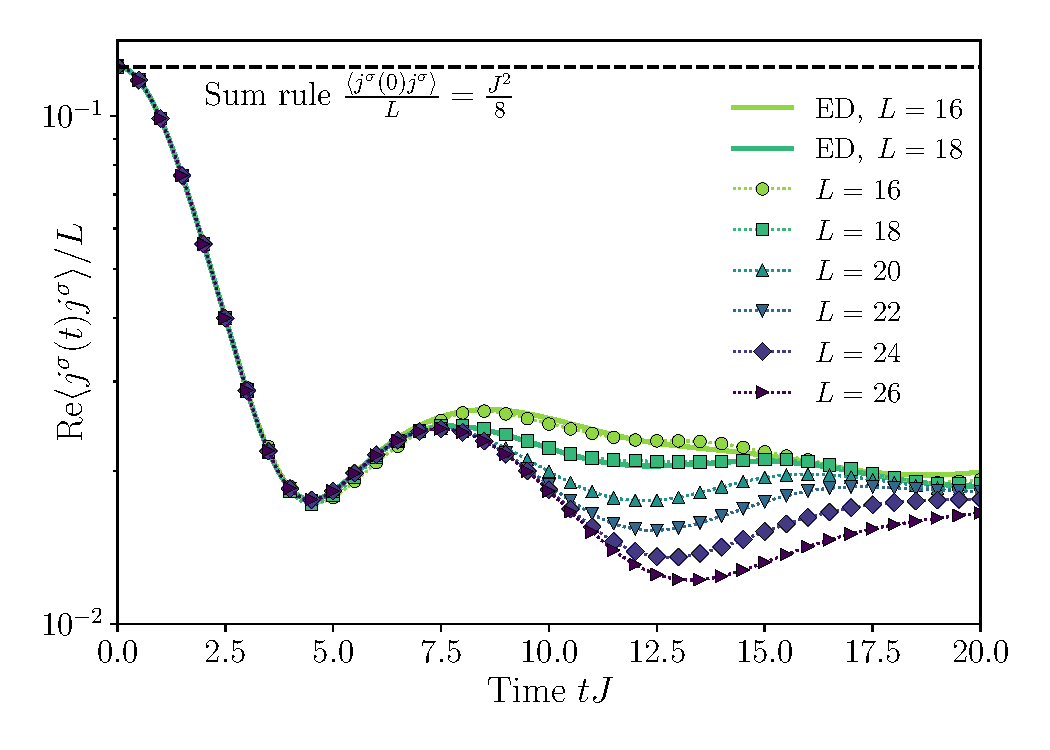
\includegraphics[width=\textwidth]{Figures/autocorr_spin_current.pdf}
	\caption{Autocorrelation function of spin current \(j_{\sigma}\) in isotropic Heisenberg model
	(\(J=1,\;\Delta=1\)), evaluated
	using Exact Diagonalization for \(L=16,\;18\) and Dynamical Quantum Typicality with Krylov propagator
	for \(L=16,\;18,\;20,\;22,\;24,\;26\). Already for a modest size of \(L=18\) lattice sites we observe
	a very good agreement between ED and DQT calculation for a single pure state. Because of eq.~\eqref{eq:dqt_bound},
	we expect this agreement to be exponentially better for larger system sizes.}
	\label{fig:spin_autocorr}
\end{figure}

